% Options for packages loaded elsewhere
\PassOptionsToPackage{unicode}{hyperref}
\PassOptionsToPackage{hyphens}{url}
%
\documentclass[
  9pt,
  ignorenonframetext,
]{beamer}
\usepackage{pgfpages}
\setbeamertemplate{caption}[numbered]
\setbeamertemplate{caption label separator}{: }
\setbeamercolor{caption name}{fg=normal text.fg}
\beamertemplatenavigationsymbolsempty
% Prevent slide breaks in the middle of a paragraph
\widowpenalties 1 10000
\raggedbottom
\setbeamertemplate{part page}{
  \centering
  \begin{beamercolorbox}[sep=16pt,center]{part title}
    \usebeamerfont{part title}\insertpart\par
  \end{beamercolorbox}
}
\setbeamertemplate{section page}{
  \centering
  \begin{beamercolorbox}[sep=12pt,center]{part title}
    \usebeamerfont{section title}\insertsection\par
  \end{beamercolorbox}
}
\setbeamertemplate{subsection page}{
  \centering
  \begin{beamercolorbox}[sep=8pt,center]{part title}
    \usebeamerfont{subsection title}\insertsubsection\par
  \end{beamercolorbox}
}
\AtBeginPart{
  \frame{\partpage}
}
\AtBeginSection{
  \ifbibliography
  \else
    \frame{\sectionpage}
  \fi
}
\AtBeginSubsection{
  \frame{\subsectionpage}
}
\usepackage{lmodern}
\usepackage{amsmath}
\usepackage{ifxetex,ifluatex}
\ifnum 0\ifxetex 1\fi\ifluatex 1\fi=0 % if pdftex
  \usepackage[T1]{fontenc}
  \usepackage[utf8]{inputenc}
  \usepackage{textcomp} % provide euro and other symbols
  \usepackage{amssymb}
\else % if luatex or xetex
  \usepackage{unicode-math}
  \defaultfontfeatures{Scale=MatchLowercase}
  \defaultfontfeatures[\rmfamily]{Ligatures=TeX,Scale=1}
\fi
\usetheme[]{Goettingen}
\usecolortheme{rose}
% Use upquote if available, for straight quotes in verbatim environments
\IfFileExists{upquote.sty}{\usepackage{upquote}}{}
\IfFileExists{microtype.sty}{% use microtype if available
  \usepackage[]{microtype}
  \UseMicrotypeSet[protrusion]{basicmath} % disable protrusion for tt fonts
}{}
\makeatletter
\@ifundefined{KOMAClassName}{% if non-KOMA class
  \IfFileExists{parskip.sty}{%
    \usepackage{parskip}
  }{% else
    \setlength{\parindent}{0pt}
    \setlength{\parskip}{6pt plus 2pt minus 1pt}}
}{% if KOMA class
  \KOMAoptions{parskip=half}}
\makeatother
\usepackage{xcolor}
\IfFileExists{xurl.sty}{\usepackage{xurl}}{} % add URL line breaks if available
\IfFileExists{bookmark.sty}{\usepackage{bookmark}}{\usepackage{hyperref}}
\hypersetup{
  pdftitle={BIOS6643 Longitudinal},
  pdfauthor={EJC},
  hidelinks,
  pdfcreator={LaTeX via pandoc}}
\urlstyle{same} % disable monospaced font for URLs
\newif\ifbibliography
\setlength{\emergencystretch}{3em} % prevent overfull lines
\providecommand{\tightlist}{%
  \setlength{\itemsep}{0pt}\setlength{\parskip}{0pt}}
\setcounter{secnumdepth}{-\maxdimen} % remove section numbering
\AtBeginSubsection{}
\AtBeginSection{}
\ifluatex
  \usepackage{selnolig}  % disable illegal ligatures
\fi

\title{BIOS6643 Longitudinal}
\subtitle{L20 Missing data}
\author{EJC}
\date{}
\institute{Department of Biostatistics \& Informatics}

\begin{document}
\frame{\titlepage}

\begin{frame}[allowframebreaks]
  \tableofcontents[hideallsubsections]
\end{frame}
\hypertarget{missing-data}{%
\section{Missing data}\label{missing-data}}

\begin{frame}{Topics for today}
\protect\hypertarget{topics-for-today}{}
\begin{itemize}
\tightlist
\item
  Addressing missing data in longitudinal studies!
\end{itemize}

\vspace{\baselineskip}

\begin{itemize}
\tightlist
\item
  Related reading: See the `Missing data' chapter in the course notes.
\end{itemize}
\end{frame}

\begin{frame}{Longitudinal models and missing data}
\protect\hypertarget{longitudinal-models-and-missing-data}{}
See the course notes (Longitudinal models and missing data) for more
detail.

There is also an informative tutorial article by Hogan et al., 2004,
Statistics in Medicine, ``Handling drop-out in longitudinal studies.''
\end{frame}

\hypertarget{introduction}{%
\section{Introduction}\label{introduction}}

\begin{frame}{Introduction}
\protect\hypertarget{introduction-1}{}
There is a wealth of research devoted to missing data, its impact on
results, and how to deal with it.

Missing data are particularly a problem for longitudinal studies because
often subjects start in the study, but for one reason or another they
dropout.

In this chapter, we first discuss how mixed models can naturally account
for missing data by taking correlation between responses into account.
We then discuss types of data that make it harder or easier to account
for missing data, and define general types of mechanisms for missingness
commonly discussed in the literature.

A few case studies are presented at the end.
\end{frame}

\begin{frame}{Mixed models and estimation in light of missing data}
\protect\hypertarget{mixed-models-and-estimation-in-light-of-missing-data}{}
Consider outcome data (\(Y\)) collected on subjects at 2 time points
(Visit 1 and 2). Three of the subjects have missing data for Visit 2.
The line just connects the averages of available data, by time point.

\begin{center}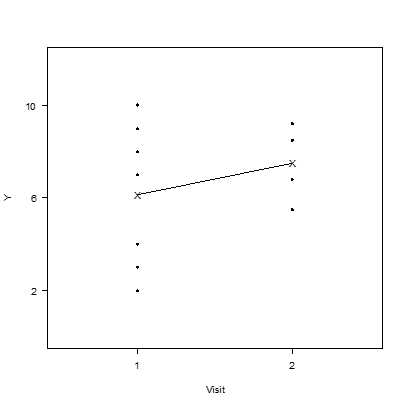
\includegraphics[width=0.7\linewidth]{figs_L20/f1} \end{center}
\end{frame}

\begin{frame}{}
\protect\hypertarget{section}{}
Now consider identifying the repeated measures within subjects (below).
The dashed lines in the left graph show the true progression for the
subjects with missing data; I have included the missing values with open
circles, although the analyst does not observe them.

\begin{center}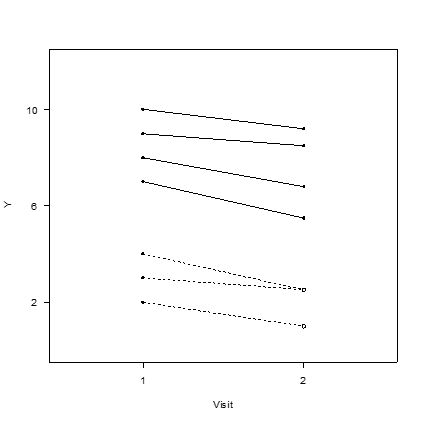
\includegraphics[width=0.7\linewidth]{figs_L20/f2} \end{center}
\end{frame}

\begin{frame}{}
\protect\hypertarget{section-1}{}
Predicted values (red) are shown below if we include a random intercept
for subjects in the model (red line connecting X's is the estimated
population average).

\begin{center}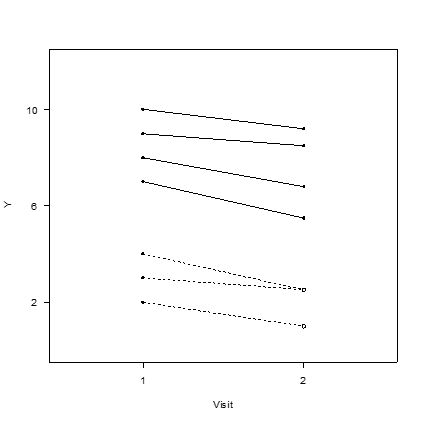
\includegraphics[width=0.7\linewidth]{figs_L20/f2} \end{center}

This illustrates that we can get accurate estimates of subject values as
well as the population-average fit in the presence of missing data if
the model is appropriate for the data.
\end{frame}

\begin{frame}{Systematic differences that are informative or not}
\protect\hypertarget{systematic-differences-that-are-informative-or-not}{}
If the subjects that had missing data for Visit 2 were systematically
different than those with complete data, then there is really no way we
get good estimates unless the observed or other data informs us about
the systematic differences.

\begin{block}{Example 1}
\protect\hypertarget{example-1}{}
\begin{center}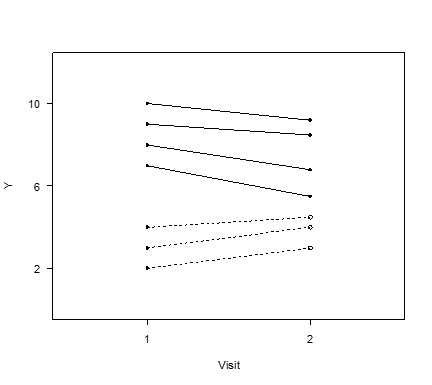
\includegraphics[width=0.7\linewidth]{figs_L20/f4} \end{center}
\end{block}

\begin{block}{Example 2}
\protect\hypertarget{example-2}{}
\begin{center}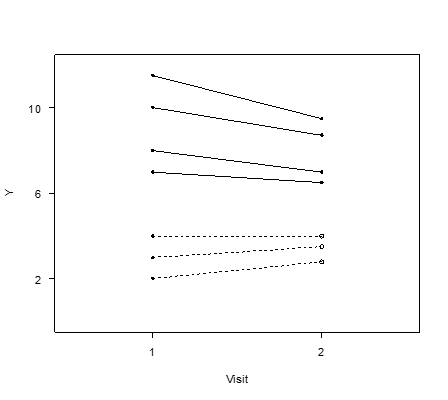
\includegraphics[width=0.7\linewidth]{figs_L20/f5} \end{center}
\end{block}
\end{frame}

\begin{frame}{}
\protect\hypertarget{section-2}{}
Two possible modeling approaches when change is related to starting
point, as in Example 2:

\begin{itemize}
\item
  Model Y2--Y1 as outcome, include Y1 as a predictor.
\item
  Use an LMM; keep both measures as outcomes, add random intercept and
  slope for time, use UN structure in G.
\end{itemize}

Unfortunately with only 2 time points, including a random slope for
visit will likely lead to a mixed model fit with a non-positive-definite
Hessian matrix and consequently some limited and/or questionable output.

The modeling approaches mentioned above become more useful and easier
when there are \(t>2\) time points.
\end{frame}

\hypertarget{missing-data-mechanisms}{%
\section{Missing data mechanisms}\label{missing-data-mechanisms}}

\begin{frame}{Missing data mechanisms}
\protect\hypertarget{missing-data-mechanisms-1}{}
Definitions involve missing response (\(Y\)) data

\begin{itemize}
\item
  Missing completely at random (MCAR)

  \begin{itemize}
  \item
    Simple
  \item
    Covariate-dependent
  \end{itemize}
\item
  Missing at random (MAR)
\item
  Missing not at random (MNAR)
\end{itemize}
\end{frame}

\hypertarget{mcar}{%
\section{MCAR}\label{mcar}}

\begin{frame}{MCAR}
\protect\hypertarget{mcar-1}{}
Simple MCAR data

\begin{itemize}
\item
  Probability that the response is missing is unrelated to any of the
  data, including the missing responses.
\item
  \(P(M_{ij}=1|Y_{(i,obs)},Y_{(i,miss)}, X_i)=P(M_{ij}=1)\), where
  \(Y_{(i,obs)}\) and \(Y_{(i,miss)}\) denote the observed and missing
  components of the responses, \(X_i\) denotes relevant predictors in
  the model, and \(M_{ij}\) is an indicator for missingness (1=missing,
  0=observed), for subject \(i\) at time \(j\).
\end{itemize}

Covariate-dependent MCAR data

\begin{itemize}
\item
  \(P(M_{ij}=1|Y_{(i,obs)},Y_{(i,miss)},X_i)=P(M_{ij}=1|X_i)\)
\item
  See Hedeker and Gibbons, 2006; Fitzmaurice et al., 2011.
\item
  A bit more realistic than simple MCAR.
\end{itemize}

MCAR is the most restrictive assumption and is probably the least likely
to hold for real data. However, one can test whether data are MCAR or
not fairly easily.
\end{frame}

\hypertarget{mar}{%
\section{MAR}\label{mar}}

\begin{frame}{MAR}
\protect\hypertarget{mar-1}{}
The next level up is MAR data, which satisfies
\(P(M_{ij}=1|Y_{(i,obs)},Y_{(i,miss)},X_i)=P(M_{ij}=1|Y_{(i,obs)},X_i)\).
Modeling MAR data can still be done somewhat easily if the model
contains the necessary variables for the observed data.

E.g., progression of lung function over time for smokers (S) and
nonsmokers (NS):

\begin{itemize}
\item
  Smokers have lower starting values and steeper drops in response over
  time compared with nonsmokers.
\item
  Smokers are more likely to dropout (40\% for S, 20\% for NS).\\
  Missingness depends on smoking status, but by including the relevant
  predictors in the model (smoking status, time and their interaction),
  we can accurately model the data.
\item
  Within smoking status groups, the probability of missingness at a
  follow-up visit is constant across subjects, and so whether or not a
  subject's response at a follow-up visit is observed does not depend on
  its potentially unobserved value.
\end{itemize}
\end{frame}

\begin{frame}{}
\protect\hypertarget{section-3}{}
When the values of the missing data are related to the chance that they
are missing (specifically, when the probability equation in the last
paragraph does not hold), the mechanism is referred to as missing not at
random (MNAR; or in some places, termed `not missing at random' or
NMAR).

For a simple example, consider a study where a health outcome is
measured over time, where subjects are more likely to dropout once they
become sick. If the health outcome measure decline for these sick
subjects but we did not observe their outcomes during this state, then
data are likely MNAR.

Unfortunately, there are no easy tests to determine whether data are MAR
versus MNAR unless some additional information becomes available (e.g.,
some of the missing responses are randomly obtained).
\end{frame}

\begin{frame}{}
\protect\hypertarget{section-4}{}
There are methods of estimation that do account for MNAR type of data,
if there is concern that data may follow that, including pattern mixture
models and selection models (e.g., see Diggle et al., 2002), and Kenward
(1998) even suggested a selection model for 2-visit data with missing
values. If there is enough uncertainty about MAR versus MNAR data,
methods for the two approaches can always both be run in a `sensitivity
fashion' to help determine how much difference it makes.

Review: are previous Examples 1 and 2 likely to be MAR or MNAR?
\end{frame}

\hypertarget{approaches-for-missing-x-data}{%
\section{\texorpdfstring{Approaches for missing \(X\)
data}{Approaches for missing X data}}\label{approaches-for-missing-x-data}}

\begin{frame}{Approaches for missing \(X\) data}
\protect\hypertarget{approaches-for-missing-x-data-1}{}
When \(Y\) is missing at random (MAR) but covariate data are complete,
then it is sufficient to use the standard linear mixed model in order to
obtain unbiased estimates, as described above. However, when \(X\) is
missing (potentially with some missing \(Y\)), standard likelihood based
methods may not be sufficient.

To address potential bias for missing \(X\) data, one might consider
other likelihood-based algorithms, such as the EM algorithm, or another
modeling approach, such as multiple imputation. Such approaches may be
able to incorporate records that involve missing \(X\) data rather than
just removing records. Although most standard procedures simply drop the
records from analysis when covariate data are missing, there are ways to
account for correlation between responses in such cases, as described
above.
\end{frame}

\begin{frame}{GEE and estimation in light of missing data}
\protect\hypertarget{gee-and-estimation-in-light-of-missing-data}{}
When using GEE associated with GzLMs, unlike mixed models that employ
more standard likelihood-based estimation methods, MAR-type data cannot
necessary be handled by simply including key predictor variables. For
GEE, a stronger assumption of MCAR is necessary in order to use typical
estimation methods. Fitzmaurice, et al.~(2011), also discuss how to
employ weighting techniques for GEE models when data are MAR.
\end{frame}

\begin{frame}{Preparation of data and specification of models in light
of missing data}
\protect\hypertarget{preparation-of-data-and-specification-of-models-in-light-of-missing-data}{}
In this section we focus on computational issues for data with missing
values when fitting linear mixed models, and how you should specify a
data set to get an accurate model fit when using computer software such
as SAS or R.

Note that which software you use makes a difference on the approach.
Here we focus on data with serial correlation that can be modeled with
an AR(1) or related structure. Including random effects such as a random
intercept are less problematic in light of missing data since each pair
of responses have the same model correlation, regardless of time between
responses. On the other hand, the AR(1) is sensitive to the time between
measurements, and so missing values need to be carefully considered.
\end{frame}

\begin{frame}{Linear mixed models in SAS and R}
\protect\hypertarget{linear-mixed-models-in-sas-and-r}{}
For unequally spaced data that is due to design or missingness, I would
generally recommend using a spatial covariance structure (e.g., spatial
power in SAS) to properly account for different gaps between
measurements.

However, you still potentially need to address the missing data issue,
i.e., just because we use a structure that accounts for gaps due to
missing data doesn't mean we've addressed potential bias in estimates
caused by the missing values.

The course notes go into more detail about how you can use a structure
like AR(1) instead of a spatial structure in light of intermittent data.
\end{frame}

\begin{frame}{}
\protect\hypertarget{section-5}{}
When specifying serial correlation in a model with no random effects,
the gls function can be used in R. Recall that missing values are
specified using `NA'. Some functions such as \textbf{gls()} or
\textbf{lme()} (from the \textbf{nlme} package) cannot process the
records with `NA' without more instruction about how to deal with them.
Specifically, telling the function to omit or exclude the records will
allow the model to be fitted.

The discrete AR(1) in R is specified by `corAR(1)' while the continuous
AR(1) is specified by `corCAR(1)'. The latter is the same as the spatial
power structure in SAS.
\end{frame}

\begin{frame}{GEEs with SAS and R}
\protect\hypertarget{gees-with-sas-and-r}{}
In SAS, PROC GENMOD, the AR(1) working structure is available to model
repeated measures over time. If responses are unequally spaced,
unfortunately spatial structures are not available to use.

However, for most data it is possible to get around this issue by
creating equal time units and then filling in the data set with missing
values, as necessary. This will work even when covariate measures, other
than time, are missing too.

For example, say data are collected on weekdays but the response and
covariates other than time are not collected on weekends.

In the data set, just include a record for every day in the month, and
put missing values in for \(Y\) and covariates on the weekend days
(other than for `day', which should be complete), and employ the AR(1)
working structure for GEE.

The fitted model will reflect the unequal spacing caused by no
collection on weekends. R has at least a couple of packages to fit GEE
models: the geeglm function within the \textbf{geepack} package is one
route, and the \textbf{gee()} function within the \textbf{gee} package
is another. However, within the default settings the correct spacing
cannot be specified when there are missing data for either approach.
\end{frame}

\hypertarget{case-studies}{%
\section{Case studies}\label{case-studies}}

\begin{frame}{Case studies}
\protect\hypertarget{case-studies-1}{}
The examples so far in this section have involved 2 repeated measures
over time. Most longitudinal data will have more time points. Although
this will probably complicate the analysis, it should allow the
researcher to better understand whether missing data is an issue, and
also to account for it in the modeling approach.

\begin{block}{Case study I: IPF data and the marginal mean}
\protect\hypertarget{case-study-i-ipf-data-and-the-marginal-mean}{}
Background. From \textbf{Strand et al., 2014}: The usual interstitial
pneumonia (UIP) pattern of lung injury may occur in the setting of
connective tissue disease (CTD), but it is most commonly found in the
absence of a known cause, in the clinical context of idiopathic
pulmonary fibrosis (IPF). Our objective was to observe and compare
longitudinal changes in pulmonary function and survival between patients
with biopsy-proven UIP found in the clinical context of either CTD or
IPF.
\end{block}
\end{frame}

\begin{frame}{}
\protect\hypertarget{section-6}{}
Percent of predicted diffusing capacity of the lung for carbon monoxide
(ppDLCO) is shown to the right, versus time since diagnosis; higher
values relate to better health. A LOESS fit to the data is also
included.

\begin{center}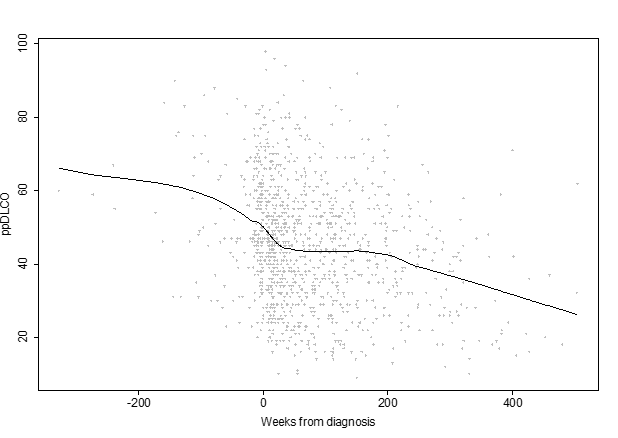
\includegraphics[width=0.7\linewidth]{figs_L20/f6} \end{center}
\end{frame}

\begin{frame}{}
\protect\hypertarget{section-7}{}
What is not implied by the plot is that data are longitudinal, with
subjects having varying number of repeated measures. Here is another
look at the data using a spaghetti plot.

\begin{center}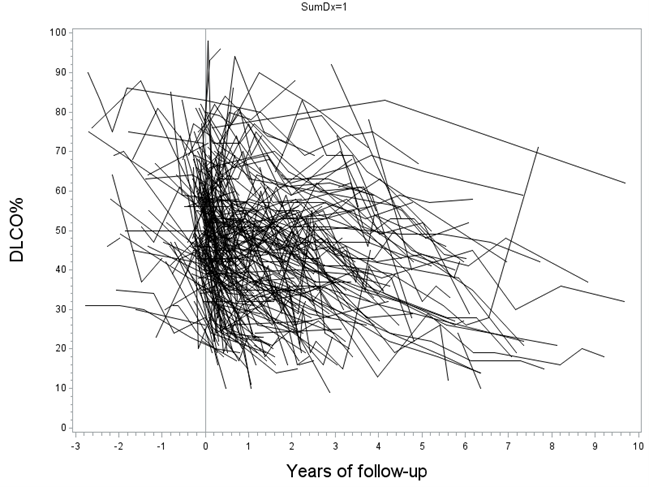
\includegraphics[width=0.7\linewidth]{figs_L20/f7} \end{center}
\end{frame}

\begin{frame}{}
\protect\hypertarget{section-8}{}
By stratifying on last observation date (\textless100 or \(\geq\) 100)
we can more clearly see the pattern:

\begin{center}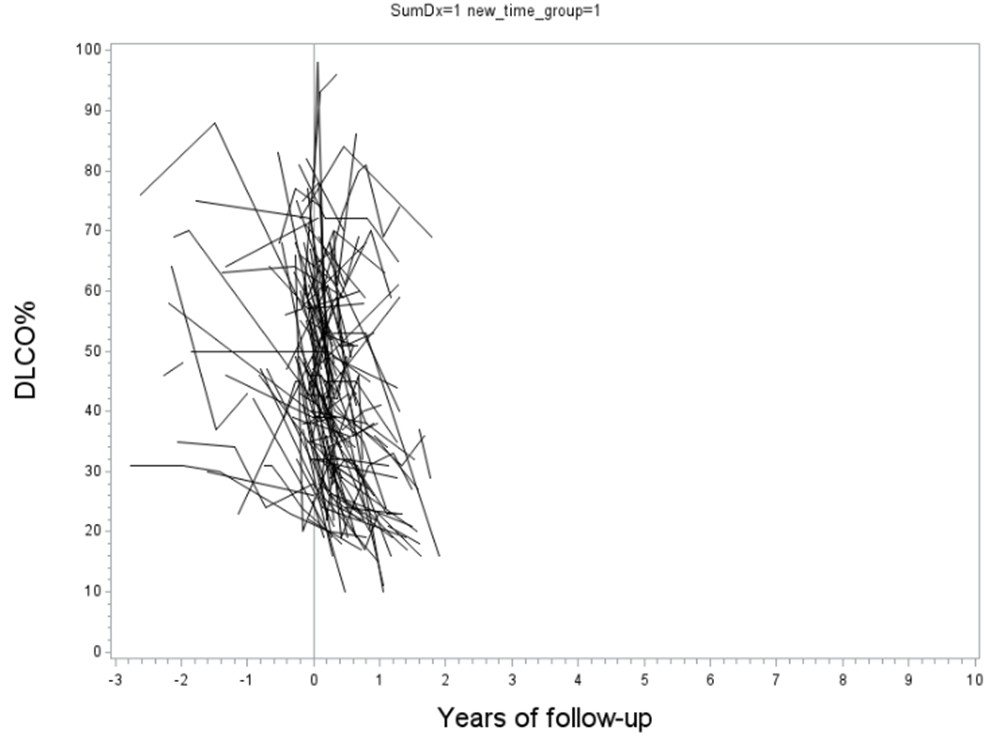
\includegraphics[width=0.7\linewidth]{figs_L20/f8} \end{center}

\begin{center}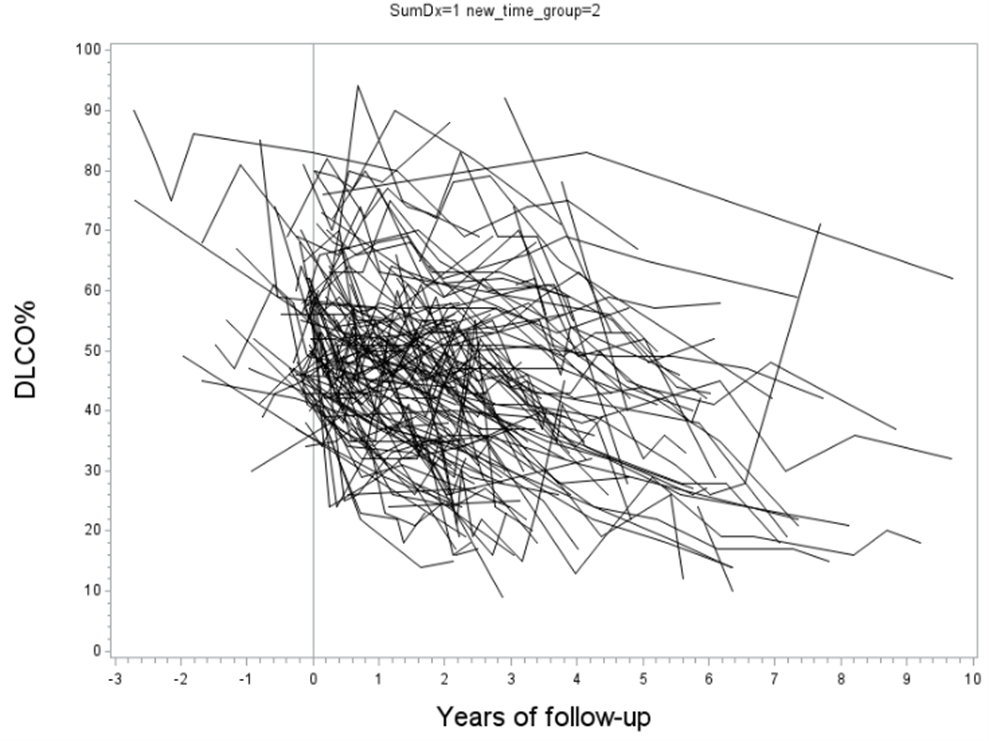
\includegraphics[width=0.7\linewidth]{figs_L20/f9} \end{center}
\end{frame}

\begin{frame}{}
\protect\hypertarget{section-9}{}
If we simply average the data over available data by time, we end up
with a convoluted function that is difficult to interpret (such as LOESS
fit on previous slide).

The inverted hump occurs because subjects who drop out early have a
large impact on the mean function, and then do not contribute to it
after 2 or so years from diagnosis; those remaining to contribute to the
function are the more robust subjects who go on for several more years
of follow up.

This raises a question of how the mean marginal function should be
defined, and whether a marginal function even makes sense.
\end{frame}

\begin{frame}{}
\protect\hypertarget{section-10}{}
If we do decide to estimate one marginal mean function, below is a
comparison of estimates based on models that assume different data
mechanisms. Here, we're estimating progression for all IPF subjects as
if all had been observed through the 10 years.

\begin{center}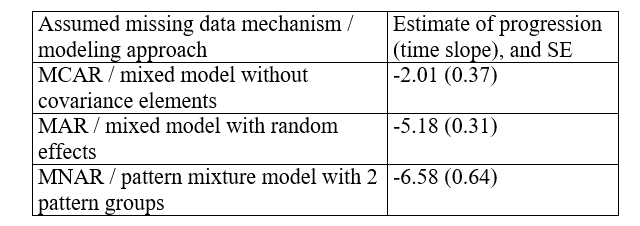
\includegraphics[width=0.7\linewidth]{figs_L20/f10} \end{center}

SAS code to derive estimates (similar to that shown in Hogan et al.,
2014) are given in the course notes.
\end{frame}

\begin{frame}{}
\protect\hypertarget{section-11}{}
The MNAR approach was derived using 2 assumed patterns, one for subjects
who dropout less than 100 weeks, and one for those \(\geq\) 100 weeks.

The estimate of -6.58\%/yr is a weighted average of the two slopes of
shown in the previous figure, where the weights are proportions of
subjects in each of the subgroups.

Another MNAR approach would be to expand the missing patterns groups to
4 or 5. (Potential student project?)

One important consideration for the marginal estimates discussed above
is over what range the estimates should be considered. The assumption
we're making is that the mean function applies to all subjects, and
predicted values are factored in even for those who die due to the
illness that causes the decline in the outcome.
\end{frame}

\begin{frame}{}
\protect\hypertarget{section-12}{}
Should all missing data be treated equally? If the outcome measures
progression of an illness, such as here, then should someone who drops
out but is still alive be treated the same as someone who dies due to
the illness being examined? If not, then estimating a marginal mean
function may not make sense.

An alternative approach is to have mean functions defined for subgroups
based on time of dropout (or possibly other factors), and then not
combine them. To the right are estimated functions for subjects observed
\textless100 weeks (solid), and \(\geq\) 100 weeks (dashed). (See Strand
et al., 2014.)

\begin{center}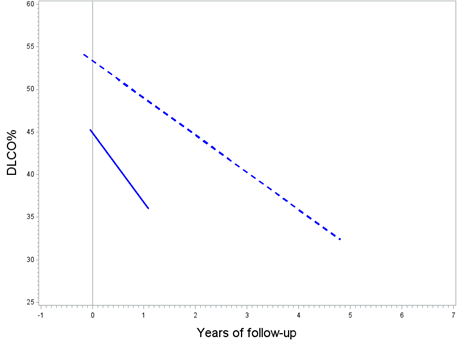
\includegraphics[width=0.7\linewidth]{figs_L20/f11} \end{center}
\end{frame}

\begin{frame}{}
\protect\hypertarget{section-13}{}
\begin{block}{Case study II: eNO and aspirin data}
\protect\hypertarget{case-study-ii-eno-and-aspirin-data}{}
Application: recall the eNO data first presented in the Graphs chapter.
Below are the data, which now includes the 6mo and 1yr time points
(eno\_1=pre challenge; eno\_2=post challenge; eno\_3=6 months after
challenge; eno\_4=1 year after challenge).

Note that there is technically only 1 day difference between the pre and
post challenge measurements. However, to allow for visual
interpretation, a spread of 10 days was used between eno\_1 and eno\_2;
otherwise data were plotted metrically for time. In the data, missing
values were represented by `.' (For R, they would be represented with
`NA'.)

The data were sorted by eno\_1 and demonstrate that those with higher
baseline eNO (indicating more inflammation) were more likely to drop out
later on, although the subject with the highest starting eNO and biggest
reaction to aspirin was a completer.
\end{block}
\end{frame}

\begin{frame}{}
\protect\hypertarget{section-14}{}
A straight mean of available data shows an increase in eNO after the
aspirin challenge, which then drops somewhat at 6 months and 1 year.
This is also apparent in the graph of individual subjects. Although
dropouts tend to occur as time goes on, there are a few cases where
subjects missed intermediate time points but actually came back. These
are represented with dashed lines (they both missed the 6mo time point).

Two questions for the reader: (1) Based on what you see, what type of
missing data mechanism would you expect the data to follow? (2) How
would you check for and handle (if applicable) the missing data?
\end{frame}

\begin{frame}{}
\protect\hypertarget{section-15}{}
\begin{center}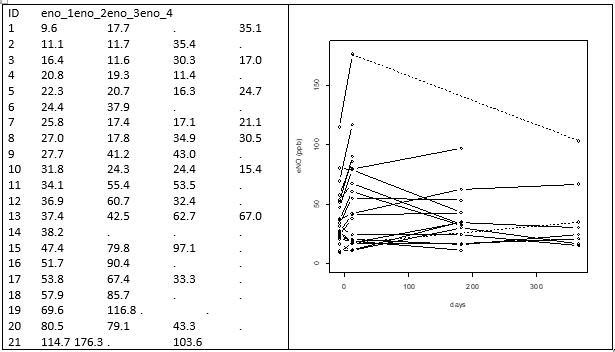
\includegraphics[width=0.7\linewidth]{figs_L20/f12} \end{center}

Supplement -- an even broader list of approaches to account for missing
data
\end{frame}

\begin{frame}{}
\protect\hypertarget{section-16}{}
Complete case (not recommended unless shown to be similar to other
approaches)

Last observation carried forward (not recommended)

All-available data approach (probably the best `standard' method)

Inverse probability weighting

Multiple imputation

MAR-type analytical approaches

NMAR-type analytical approaches
\end{frame}

\hypertarget{inverse-probability-weighting}{%
\section{Inverse probability
weighting}\label{inverse-probability-weighting}}

\begin{frame}{Inverse probability weighting (IPW)}
\protect\hypertarget{inverse-probability-weighting-ipw}{}
Upweights subjects that tend to dropout more. Create weights from an
initial logistic regression (outcome = was response observed, yes or
no).

Plug weights into final model to upweight/downweight records, by using
the `weight' statement.

To allow weights to have correct impact, do not model correlation
between measures within a subject (use `VC' structure), but also use
empirical SE's to help account for model misspecficiation.
\end{frame}

\hypertarget{multiple-imputation}{%
\section{Multiple imputation}\label{multiple-imputation}}

\begin{frame}{Multiple imputation}
\protect\hypertarget{multiple-imputation-1}{}
Impute missing data based on available information. Repeat `\(k\)' times
so uncertainty in the imputation can be factored into SE's.

Works better when you have `almost complete' data for subjects at a
given time, but perhaps just missing 1 or 2 variables.

\begin{block}{Case study III: The COPDGene Study}
\protect\hypertarget{case-study-iii-the-copdgene-study}{}
Outcomes for subjects with COPD observed over time; Phase 1: 0 years,
Phase 2: 5 years, Phase 3: 10 years (approximately). But there is some
loss to follow up (dropouts, deaths, latecomers).
\end{block}
\end{frame}

\begin{frame}{MAR-type analysis}
\protect\hypertarget{mar-type-analysis}{}
Recall: with MAR-type data, the probability of missingness depends only
on predictors and observed responses.

Identify the predictors (and their interactions with time) that are
likely to cause the most problems. Add them to the model.

Smoking status and race are known demographics to have differential
dropout. Add them, plus interactions, to model. If their inclusion does
not change things, can simplify.
\end{frame}

\begin{frame}{}
\protect\hypertarget{section-17}{}
We know current smokers tend to dropout more. So add smoking group and
smoking group*time to account for differential dropout by smoking
status. Stratifying analyses by GOLD group also reduces potential bias
caused by MAR-type data.

\begin{center}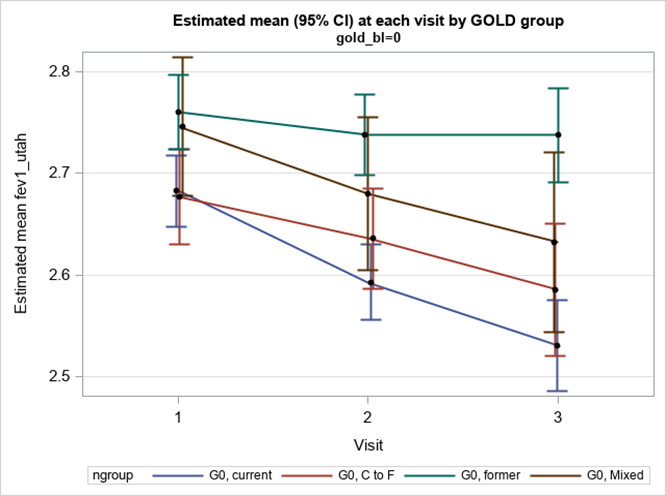
\includegraphics[width=0.7\linewidth]{figs_L20/f13} \end{center}
\end{frame}

\begin{frame}{NMAR-type analysis}
\protect\hypertarget{nmar-type-analysis}{}
Pattern mixture modeling. Actual progression estimates can be obtained
by identifying responses for `important' missing data patterns, and then
using a weighted average of these to obtain a marginal mean estimate.

For COPDGene, there are a limited number of patterns over time (P1,
P1P2, P1P3, P1P2P3), which makes it a little easier to examine. This is
a reasonable approach if the patterns only depend on time.

For both GOLD 1 and 3 groups, there do not appear to be big differences
between the response pattern groups, suggesting MAR-type approaches may
be o.k. (at least for these groups).

\begin{center}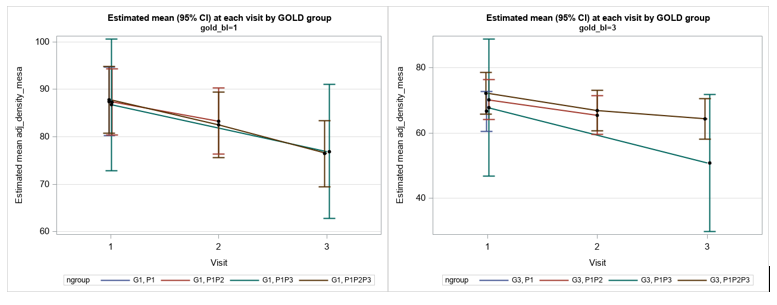
\includegraphics[width=0.7\linewidth]{figs_L20/f14} \end{center}
\end{frame}

\begin{frame}{}
\protect\hypertarget{section-18}{}
If patterns do differ enough, a weighted average can be taken over the
groups to obtain one overall estimate. Results can also just be kept
separate.

There might be other grouping to consider (other than just time), such
as race or smoking status groups.

For NMAR-type data, we are trying to uncover latent groupings suggested
by the data. But it is really hard to check assumptions since we need to
see the unobserved responses to check it.

We have also performed IPW and multiple imputation approaches for these
data. If you are interested in seeing these programs, e.g., to see if it
may apply to your project data, let me know. Also, for more detail on
these methods and how they relate to missingness assumptions, see
\textbf{Fitzmaurice et al., 2011, 2nd ed., Applied Longitudinal
Analysis}.

Another good reference: \textbf{Hogan et al., 2004; 23:1455-1497},
Handling drop-out in longitudinal studies. Statistics in Medicine. This
is posted on Canvas (see Supplement module).

\begin{itemize}
\item
  They walk through examples that demonstrate analyses under different
  missingness assumptions.
\item
  They show that adding random intercepts and slope for time for
  subjects also takes care of missing data under the MAR assumption.
\end{itemize}
\end{frame}

\begin{frame}{General thoughts}
\protect\hypertarget{general-thoughts}{}
Should deaths and dropout for other reasons be distinguished? What are
the implications if we just pool it all together?

Joint longitudinal and survival models can also be used to account for
missing data due to death, or for dropout more generally. This involves
constructing a likelihood that includes both facets, e.g., a linear
mixed model plus a survival model.
\end{frame}

\end{document}
